\documentclass[11pt,spanish,listoffigures]{tfgetsinf}
\usepackage[utf8]{inputenc} 

%%%%%%%%%%%%%%%%%%%%%%%%%%%%%% PORTADA %%%%%%%%%%%%%%%%%%%%%%%%%%%%%%

\title{Implementación de un API Gateway para una arquitectura de microservicios}
\author{Alejandro Carrión Sanmartín}
\tutor{Patricio Letelier Torres}
\curs{2020-2021}

%%%%%%%%%%%%%%%%%%%%%%%%%%%%%% PALABRAS CLAVE %%%%%%%%%%%%%%%%%%%%%%%%%%%%%%

\keywords{????, ?????????} % Paraules clau 
         {?????, ???} % Palabras clave
         {?????, ?????} % Key words

\begin{document}

%%%%%%%%%%%%%%%%%%%%%%%%%%%%%% RESUMEN %%%%%%%%%%%%%%%%%%%%%%%%%%%%%%

\begin{abstract}[spanish]
????
\end{abstract}
\begin{abstract}[catalan]
????
\end{abstract}
\begin{abstract}[english]
????
\end{abstract}

\mainmatter

%%%%%%%%%%%%%%%%%%%%%%%%%%%%%% INTRODUCCIÓN %%%%%%%%%%%%%%%%%%%%%%%%%%%%%%

\chapter{Introducción}

El uso de arquitecturas de microservicios es una práctica ya establecida hoy en día en el mundo del desarrollo de \emph{software}. Esta consiste en la construcción de servicios independientes, ejecutados en procesos diferentes, que se encargan de realizar funciones concretas y que trabajan de forma conjunta para lograr el objetivo u objetivos globales de la aplicación. Los beneficios que otorga este enfoque frente a la aproximación tradicional monolítica son muchos y muy variados. Algunos de ellos son:

\begin{itemize}

	\item \textbf{Uso de diferentes tecnologías}.
Cada microservicio puede estar construido con una tecnología diferente y puede utilizar diferentes mecanismos de persistencia.

	\item \textbf{Maniobrabilidad en los despliegues}.
Ante cualquier cambio no es necesario desplegar la aplicación entera, solamente los microservicios implicados.

	\item \textbf{Escalabilidad y mantenibilidad}.
Los microservicios, y la separación funcional que otorgan, facilitan el escalado de las diferentes partes de la aplicación de manera independiente. Lo mismo sucede con el mantenimiento, pudiendo crear equipos especializados.

\end{itemize}

Se puede obtener más información acerca de los microservicios en el artículo de James Lewis y Martin Fowler titulado ''\emph{Microservices}'' \cite{LewisAndFowler}.

Por contraparte, este tipo de arquitecturas aumentan la complejidad del desarrollo en algunos aspectos concretos como pueden ser el versionado de los microservicios o la coordinación de las comunicaciones entre ellos. Es aquí donde entra este trabajo, pues está enfocado a paliar otra de sus desventajas: la exposición de múltiples puntos de entrada al \emph{backend}. Para ello se pretende realizar un \emph{API Gateway}.

Un \emph{API Gateway}, o \emph{Gateway} para abreviar, se entiende como un componente que se interpone entre la interfaz de usuario (frontend) de una aplicación y los servicios en los que se basa (\emph{backend}). Actúa como intermediario y es el único punto de entrada al mencionado \emph{backend}. Además, es habitual que realice tareas de autenticación, monitorización u orquestación.

Como se aprecia en la definición anterior, el uso de un \emph{Gateway} no queda restringido a arquitecturas de microservicios, también puede ser utilizado en monolíticas, si bien constituye una parte fundamental en las primeras. En estas, consigue ocultar los pequeños servicios que componen la aplicación y permite tener varias instancias de ellos en ejecución al mismo tiempo. La figura \ref{figura:gateway_o_no} muestra la comparativa de arquitecturas de microservicios cuando se utiliza un \emph{Gateway} y cuando no.

\begin{figure}[ht]
	\centering
	\label{figura:gateway_o_no}
	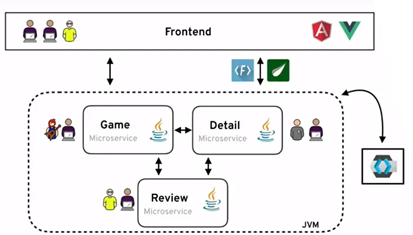
\includegraphics[width=0.45\textwidth]{images/arquitecturaMicroserviciosBasica}
	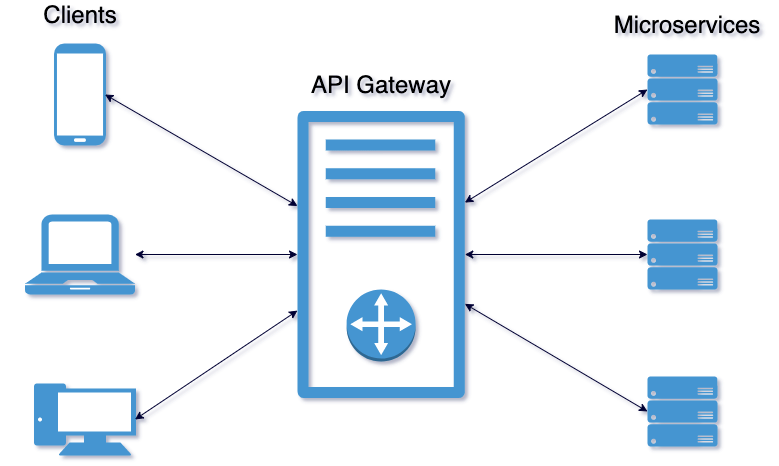
\includegraphics[width=0.45\textwidth]{images/arquitecturaMicroserviciosConGateway}
	\caption{Arquitectura de microservicios básica frente a una con \emph{API Gateway}. Imágenes de \url{https://www.adictosaltrabajo.com/2020/05/27/introduccion-al-api-gateway-pattern}.}
\end{figure}

\section{Motivación}

Este proyecto surge en el contexto de una práctica en empresa. El autor del mismo ha formado parte del equipo de \emph{I+D+i} de la compañía \emph{ADD Informática} durante el periodo de un año. \emph{ADD} es una empresa española que se dedica a desarrollar y comercializar un \emph{software} de gestión geriátrica llamado \emph{ResiPlus} \cite{ResiPlus}. Actualmente cuenta con casi cien trabajadores, es líder del mercado nacional y se encuentra en proceso de expansión internacional.

La temática del trabajo es el desarrollo de un \emph{API Gateway} para una aplicación con arquitectura de microservicios. Esta fue elegida debido a la relación que guarda con el desempeño del autor en la empresa comentada en el párrafo anterior. Por otro lado, el desarrollo a llevar a cabo le va a otorgar una visión más global de la aplicación sobre la que se trabaja así como aumentar el nivel de conocimiento acerca de la misma con la motivación de seguir contribuyendo al proyecto por mucho tiempo más. Por último, la tecnología a utilizar, \emph{.NET Core}, es de su interés y aspira así a crecer como desarrollador de ese \emph{framework}.

En cuanto a la motivación de la empresa, esta quiere dar la posibilidad de aprovechar, en cierta medida, el trabajo realizado y a realizar por el autor del documento dentro del marco de trabajo de la entidad, viéndose esta beneficiada también.

\section{Objetivos}

Este proyecto pretende resolver un problema real. Este consiste en otorgar a una aplicación con arquitectura de microservicios la capacidad de ocultarlos, así como permitir la ejecución simultánea de más de una instancia de los mismos. Cabe destacar que la aplicación en cuestión se encuentra todavía en fase de desarrollo y que el \emph{API Gateway} que se va a realizar como solución es un punto clave en su arquitectura. A raíz de lo comentado se obtienen los siguientes objetivos sobre la aplicación en construcción:

\begin{itemize}

	\item \textbf{Ocultar los microservicios} de forma que la interfaz de usuario no acceda directamente a estos por motivos de seguridad.
	
	\item Permitir la \textbf{instanciación múltiple} de los microservicios que, a su vez, tiene por objetivos:
		\begin{itemize}
		
			\item Conseguir que la aplicación sea \textbf{tolerante a fallos} gracias a la posibilidad de tener un mismo microservicio desplegado en máquinas diferentes.
			
			\item \textbf{Aumentar la eficiencia} al poder crear o parar instancias dinámicamente según el tráfico que reciba la aplicación.
			
		\end{itemize}

\end{itemize}

\section{Estructura del documento}

?????

%%%%%%%%%%%%%%%%%%%%%%%%%%%%%% CONTEXTO TECNOLÓGICO %%%%%%%%%%%%%%%%%%%%%%%%%%%%%%

\chapter{Contexto tecnológico}

En la actualidad existen en el mercado muchas aplicaciones y servicios que resuelven problemas parecidos al planteado. Algunos de estos productos \emph{software} son de pago, otros gratuitos e incluso algunos de código abierto. Se comentan los más relevantes a continuación.

\section{\emph{Amazon API Gateway}}
\emph{Amazon API Gateway} \cite{Amazon} es
	
\section{\emph{Kong}}
Tal y como dice su página web, \emph{Kong} \cite{Kong} es el \emph{API Gateway} más conocido. Se trata de una herramienta gratuita optimizada para microservicios, concebida para ser altamente escalable y que posee un gran número de \emph{plugins} desarrollados por la propia compañía y por su comunidad, que es bastante grande al ser una aplicación tan popular. Además, actualmente es utilizado por grandes empresas como \emph{Intel}, \emph{Ferrari} o \emph{Yahoo!}.
	
\section{\emph{Apigee}}
\emph{Apigee} \cite{Apigee} es
	
\section{\emph{Tyk}}
\emph{Tyk} \cite{Tyk} es
	
\section{\emph{Ocelot}}
\emph{Ocelot} \cite{Ocelot} es
	
\section{\emph{YARP}}
\emph{YARP} \cite{YARP} es

%%%%%%%%%%%%%%%%%%%%%%%%%%%%%% ANÁLISIS DEL PROBLEMA %%%%%%%%%%%%%%%%%%%%%%%%%%%%%%

\chapter{Análisis del problema}

?????

\section{Especificación de requisitos}

?????

\section{Soluciones posibles}

?????

\section{Solución propuesta}

?????

\section{Plan de trabajo y metodología}

?????

%%%%%%%%%%%%%%%%%%%%%%%%%%%%%% DISEÑO DE LA SOLUCIÓN %%%%%%%%%%%%%%%%%%%%%%%%%%%%%%

\chapter{Diseño de la solución}

?????

\section{Arquitectura del sistema}

?????

\section{Diseño detallado}

?????

\section{Tecnología utilizada}

?????

\section{Mantenimiento y gestión de versiones}

?????

%%%%%%%%%%%%%%%%%%%%%%%%%%%%%% DESARROLLO DE LA SOLUCIÓN %%%%%%%%%%%%%%%%%%%%%%%%%%%%%%

\chapter{Desarrollo de la solución}

?????

%%%%%%%%%%%%%%%%%%%%%%%%%%%%%% PRUEBAS %%%%%%%%%%%%%%%%%%%%%%%%%%%%%%

\chapter{Pruebas}

?????

%%%%%%%%%%%%%%%%%%%%%%%%%%%%%% CONCLUSIONES %%%%%%%%%%%%%%%%%%%%%%%%%%%%%%

\chapter{Conclusiones}

?????

%%%%%%%%%%%%%%%%%%%%%%%%%%%%%% BIBLIOGRAFÍA %%%%%%%%%%%%%%%%%%%%%%%%%%%%%%

\begin{thebibliography}{10}

\bibitem{LewisAndFowler}
	Artíclo de J. Lewis y M. Fowler acerca de los microservicios.
	\newblock Disponible en:\\
	\url{https://martinfowler.com/articles/microservices.html}

\bibitem{ResiPlus}
	Página web de \emph{ADD Informática} y su producto \emph{ResiPlus}:\\
	\url{https://addinformatica.com}

\bibitem{Amazon}
	Documentación oficial de \emph{Amazon API Gateway}:\\
	\url{https://aws.amazon.com/es/api-gateway}
	
\bibitem{Kong}
	Documentación oficial de \emph{Kong}:\\
	\url{https://konghq.com/kong}
	
\bibitem{Apigee}
	Documentación oficial de \emph{Apigee}:\\
	\url{https://cloud.google.com/apigee}
	
\bibitem{Tyk}
	Documentación oficial de \emph{Tyk}:\\
	\url{https://tyk.io}

\bibitem{Ocelot}
	Documentación oficial de \emph{Ocelot}:\\
	\url{https://ocelot.readthedocs.io/en/latest}

\bibitem{YARP}
	Documentación oficial de \emph{YARP}:\\
	\url{https://microsoft.github.io/reverse-proxy}

\end{thebibliography}

\end{document}
